\part{Desenvolvimento} \label{sec:parte2}

Nesta parte do documento será descrito como cada carro e nuvem foram construídos (Seção \ref{sec:construcao}), os obstáculos encontrados no desenvolvimento e utilização dos equipamentos (Seção \ref{sec:obstaculos}) e o modelo de controle construído (Seção \ref{sec:recorrencia}).

\section{Construção e Uso de Serviços e Equipamentos} \label{sec:construcao}

	\subsection{Carro Robô $ \mathcal{A} $}
		A construção do carro $ \mathcal{A} $ se baseou-se num sistema de sensores e atuadores que realiza leituras do ambiente por meio de interrupções de sistema e o envio desses dados para a nuvem. Tais dados são processados e retornados para o carro para assim ser realizado a atuação apropriada à situação segundo os cálculos do controle proporcional situado na nuvem.

		Ele possui dois sensores fototransistores na sua dianteira (Figura \ref{fig:robot_foto} na Seção Anexo) para detectar as faixas que orientam o carro e dois sensores encodificadores de rotação (Figura \ref{fig:robot_encoder} na Seção Anexo) para controle de velocidade/rotações.

		Além desses sensores, o carro é composto pois dois motores de corrente-contínua, dois \textit{pack} de pilhas e um NodeMCU junto com seu \textit{motor shield} e \textit{protoboard} para confecção do circuito elétrico, como mostrado na Figura \ref{fig:robot} na Seção Anexo.  
        

		%\subsubsection{Programação}
			O carro não possui nenhum tipo de processamento importante, sendo seu propósito único de leitura de sensores e atuação implicando numa programação simples de conexão com a nuvem, leitura, tratamento e envio dos dados e por fim sua atuação.

			A leitura do \textit{encoder} é feito por interrupção sistêmica no qual, a cada \textit{trick} alterado, o sensor realiza uma interrupção para incrementar o valor do grau de rotação naquele intervalo de tempo $t$. Tais detalhes serão explicados na respectiva seção da descrição do controle na nuvem, na Seção {sec:nuvem}.

			A detecção de faixa é feita por meio de interrupção de sistema gerando um procedimento de emergência de envio de dados para a nuvem a fim de obter resposta mais apropriada para a situação.


	\subsection{Nuvem} \label{sec:nuvem}

		O servidor foi desenvolvido utilizando linguagem de programação Python versão 2.7 que possui todos os artefatos necessários para a construção e utilização de uma aplicação com \textit{socket} para comunicação com aplicações externas.

		A nuvem recebe os dados lidos pelos sensores do carro a cada instante de tempo, definido como $30$ milissegundos, processa-os e responde o carro com os devidos comandos que ele deverá realizar sobre a situação imposta. Essa estratégia de arquitetura faz com que o processamento realizado seja inteiramente pela nuvem sendo a configuração de velocidade e de controle proporcional de execução do carro na pista sejam todas definidas via nuvem.

		%O teste de controle proporcional descrito na Análise Teórica do trabalho baseou-se na situação de que, caso encontre a faixa em algum lado do carro, a respectiva roda teria sua velocidade reduzida a ponto de que o carro possua a velocidade angular (Seção \ref{sec:velocidade_angular}) correta em cada roda para realizar a curva. Entretanto, os motores necessários não possuíam torque suficiente para o carro construído, impedindo este de realizar as movimentações necessárias como descrito na Seção \ref{sec:problema_motor}.
		
		%De forma a contornar este problema, construiu-se outra estratégia de controle proporcional que respeitasse o tempo de atuação que motor necessita para o funcionamento prático. 
        O algoritmo necessita de duas funções especiais para concluir seus cálculos sendo elas o Cálculo Proporcional (Algoritmo \ref{alg:control}) e o Cálculo de Rotação (Algoritmo \ref{alg:spin}). O primeiro algoritmo utiliza do controle P para gerar um valor de erro em relação à posição perfeita. Dado a posição atual $\Delta \Phi$ e a referência esperada $reference$, calcula-se a proporção de erro. Caso a referência seja o propósito de parar o motor, o erro 
        %será multiplicado pelo valor constante $10$ que 
        gerará um erro negativo o suficiente para solicitar a parada total do motor requerido. Obtido o erro proporcional, é feito o cálculo de velocidade do motor a fim de que tenha controle fechado sobre sua atuação. $erro = 0$ indica que o motor está na velocidade ideal. Valores positivos indicam que a potência do motor dever aumentada a fim de aproximar do requerido e negativo possui a ideia de decremento.

		\begin{algorithm}[H]
			\caption{Cálculo da proporção do erro em relação à posição referência.} \label{alg:control}
			\begin{algorithmic}[1]
				\Function{proprortion}{$\Delta \Phi, reference$}
					\State $position \gets \Delta \Phi;$
					\State $perfect\_position \gets reference; $
					\State $proportion \gets perfect\_position - position;$
					\State $error\_value \gets proportion * K_p;$
					\State \Return $error\_value;$
				\EndFunction
			\end{algorithmic}
		\end{algorithm}

		\begin{algorithm}[H]
			\caption{Cálculo da proporção de rotação dos motores sobre controle de malha fechada.} \label{alg:spin}
			\begin{algorithmic}[1]
				\Function{motors\_spin}{$\Phi, error, \Lambda$}
					\If {$\Lambda = NOT\_VISIBLE$}
							\State $rotation \gets (error * \Call{abs}{max\_rotation\_motor - rotation}) / 100$;
						\Else
							\State $rotation \gets - max\_rotation\_motor$;
					\EndIf
					
					\If {$rotation > MAX$}       \Comment{Verify if PWM value is in correct interval}
							\State $rotation \gets MAX$;
						\ElsIf {$rotation < MIN$}
							\State $rotation \gets MIN$;
					\EndIf

					\State \Return $rotation$;
				\EndFunction
			\end{algorithmic}
		\end{algorithm}

		Conhecido as funções básicas, é possível descrever o funcionamento do algoritmo de controle (Algoritmo \ref{alg:nuvem}). Ele receberá por parâmetro os valores de tempo, visualização de faixa do lado esquerdo e direito respectivamente, e somatório de \textit{tricks} de cada lado do carro, sendo respectivamente $ t, \lambda_l, \lambda_r, \phi_l, \phi_r $ suas variáveis. Cada procedimento descrito no algoritmo deverá ser processado para cada motor separadamente.

		O primeiro passo é o cálculo do deslocamento de cada motor no intervalo de tempo. Com o deslocamento, têm-se todos os dados de distância percorrido pelo carro. Verificando se o carro encontra-se sobre uma faixa, verifica-se seu erro proporcional. Caso o carro esteja sobre a faixa, o respectivo motor deverá parar enquanto o outro continua sua velocidade anteriormente estipulada. A partir do momento que sai da visualização de faixa, o controle proporcional inicia-se novamente para calcular a potência requerida ao motor para conseguir inércia suficiente para deslocar e chegar à velocidade angular requerida que é dada por $reference$.

		Tendo o erro referencial, calcula-se o valor de PWM pela função $motors\_spin$ e todos os dados relevantes da execução são salvos fisicamente em arquivo físico. Ao final, os novos valores de potência são enviados aos motores para que seja realizada a sua atuação e em seguida uma nova leitura dos sensores.

		\begin{algorithm}[H]
			\caption{Controle Proporcional em Nuvem.} \label{alg:nuvem}
			\begin{algorithmic}[1]
				\Procedure{proportional\_control}{$ t, \lambda_l, \lambda_r, \phi_l, \phi_r $}
					\State $\Delta \Phi \gets \Phi_{i} - \Phi_{i-1};$      \Comment{Angular displacement}

					\If {$\Lambda$}
							\State $error \gets $\Call{proportion}{$\Delta \Phi, reference$};
						\Else
							\State $error \gets $\Call{proportion}{$\Delta \Phi, 0$};
					\EndIf

					\State \Call{motors\_spin}{$\Phi, error, \Lambda$};
					\State \Call{save\_datas}{$t, rotation, \Phi$};
					\State \Call{send\_datas}{$rotation$};
				\EndProcedure
			\end{algorithmic}
		\end{algorithm}

		sendo:

		\begin{description}
			\item [$t$:] Instante de tempo da leitura dos sensores;
			\item [$\lambda$:] Leitura do respectivo sensor fototransistor indicando existência visual de faixa de cada lado do carro. Sendo $\Lambda$ representando operações em cada lado (esquero e direito), separadamente;
			\item [$\phi$:] Leitura dos \textit{tricks} de cada motor. Com $\Phi$ representando operações em cada lado (esquero e direito), separadamente.
		\end{description}

	\subsection{Carro Robô $ \mathcal{B} $}
		O carro robô $ \mathcal{B} $ é equipado com os mesmo equipamentos, com exceção do sensores fototransistores. Sua única função é se conectar com a nuvem mostrando sua identificação como carro com etiqueta $ \mathcal{B} $, receber o mapa do trajeto gerado pelo $ \mathcal{A} $ e executá-lo de forma a tentar reproduzir o trajeto.

		%\subsubsection{Programação}
			%Primeiramente utilizou-se da técnica mais simples que baseia-se na única tarefa de reproduzir os valores de PWM obtidos pelo carro $ \mathcal{A} $. Mas como essa abordagem de controle é do tipo de malha aberta, o carro ficaroa totalmente desgovernado, já que os valores não representarão de fato os movimentos realizados pelo primeiro utilizando este método.

			%Utilizou-se das leitura dos \textit{encoders} para auxiliar no controle de velocidade do carro a fim de criar um intervalo de confiança mais próximo de reprodução do carro $ \mathcal{A} $. 



\section{Análise dos Componentes e Obstáculos} \label{sec:obstaculos}
	Realizado a montagem dos componentes no carro, foi realizado testes com cada componente a fim de verificar a usabilidade de cada um e suas características físicas de funcionamento. Sendo assim, achou-se necessário descrever previamente os obstáculos obtidos com cada componente a serem considerados na construção controle proporcional do carro.

	\subsection{Atuadores e suas Caixas de Reduções} \label{sec:problema_motor}
		% Ele não conseguir para no tempo certo
        \subsubsection{Tempo de Atuação}
			Após realizados alguns testes com os motores, percebeu-se que eles possuem um pequeno atraso de resposta de resposta aos comandos. 
            
            Isso foi comprovado no teste de ação do carro ao perceber a presença de uma faixa. Quando o carro se depara com ela, indicando que deveria iniciar o processo de curva, as ações de alteração de velocidade ou mesmo de parada do motor não aconteciam num intervalo de tempo necessário para que o carro consiga de fato continuar dentro de sua trajetória. 

			A primeira hipótese considerada foi a latência gerada pela comunicação sem-fio na arquitetura distribuída. Entretanto, realizou-se novos testes com o sistema de controle situado totalmente no processador local do carro e o problema continuou persistindo, refutando a ideia da latência.

		\begin{comment}
		% torque suficiente para baixas rotações}
		% peso do carrinho?}
		\subsubsection{\todo{peso} da Estrutura contra Torque dos Motores}
			Além do problema do atraso do tempo de atuação, percebeu-se que o carro possui um \todo{peso} elevado em comparação à força de torque inicial que os motores acoplados a ele possuem, criando assim uma resistência maior para partida dos motores. 
			Em outras palavras, isso implica que o motor não possui torque suficiente para movimentar o carro em baixas rotações, necessitando de um valor alto de corrente para dar o torque inicial. 
			Como o carro é relativamente pesado para o motor, automaticamente a intensidade de corrente de partida aumenta para suprir a necessidade de movimentação, mas tal atuação não tem resultados positivos. 
			Motores de corrente de contínua não possui um controle de rotação e isso gera pulsos descontrolados no carro no qual o controle não consegue gerenciar bem os movimentos do carro criando assim uma trajetória complexa já pro carro $ \mathcal{A} $, aumentando ainda mais a dificuldade de reprodução do carro $ \mathcal{B} $.

			%Nas experiências com os motores, quando o carro conseguia vencer a inércia, a potência acionada ao motor era tamanha que o carro perdia o controle da velocidade acelerando o carro mais que o desejado tornando o mapa gerado pela aprendizagem mais caótico que o o esperado pelo projeto. Isso também é causado pela falta de força suficiente para mover o carro deste porte.

		\end{comment}
        
		%encoder
		\subsubsection{Controle de Velocidade Utilizando Encoder} \label{sec:problema_encoder}
        	Mesmo utilizando o \textit{encoder} para realizar o controle de velocidade, com base nos cálculos da Seção \ref{sec:encoder}, só é possível detectar movimento após $0,5105$ centímetros percorridos o que implica que, para o cálculo de velocidade do carro com mais precisão, ele precisaria andar numa velocidade maior para que obtivesse mais \textit{tricks} por intervalo de tempo.

			Isso pois, como os intervalos de tempo para cálculo e envio à nuvem são pequenos ($ 30 ms $), o cálculo da velocidade é dificultado pois taxa de \textit{tricks} por intervalo de tempo é pequena, cerca de 1 à 2, por tempo, impedindo de um controle de velocidade mais preciso.


		\subsubsection{Partida e Aceleração dos Motores}
			Nos teste com os motores e suas respectivas caixas, para que o carro conseguiesse vencer a inércia inicial, deveria injetar uma potência alta nos motores que o carro perdia o controle de direção por causa de sua brusca aceleração. Entretanto, a potência é alta o suficiente para desorientar o carro na sua aceleração.%Além do descontrole, foi percebido que o carro necessitava de altos valores de tensão para que conseguisse iniciar as rotações.

			O problema do descontrole gerado pela aceleração é que ao vencer sua inércia e iniciar a sua aceleração, o controle possui um certo atraso para detectar o início do movimento e gerenciar, logo em seguida, a velocidade requerida segundo a aceleração atual. Como mencionado em \ref{sec:problema_encoder}, o encoder não possui uma precisão fina sobre velocidade em taxas de tempo pequenas. Dessa forma, nessas acelerações o carro perde o controle ou excede a distância segura a ser percorrida.

		% dois packs de pilhas pesaram o motor}
		%\subsubsection{Uso de dois \textit{packs} de pilha}
			A relação de atuação e corrente dos motores seriam resolvidos ao adicionar mais corrente aos motores adicionando mais \textit{pack} de pilhas em paralela ao primeiro, por exemplo. Entretanto, realizou-se testes com \textit{pack} adicional para fornecer maior alimentação mas não obteve melhores resultados nos atuadores.

			Tanto com um e dois \textit{packs} de pilha, houve momentos que o controle colocou potência máxima nos motores com os dois \textit{packs} de pilhas acoplados ao carro e mesmo assim os motores não possuíam torque suficiente para dar a partida no carro, aumentando ainda mais a questão sobre o nível da resistência dos trens de engrenagens das caixas de reduções sobre a sua partida inicial.

		\begin{comment}
			% falar sobre a corrente de cada motor}
			Para confirmar todas essas hipóteses de que os motores não possuíam torque suficiente para move-lo, realizou-se testes de corrente em cada motor verificando se as pilhas foram devidamente suficientes para o sistema de motores. Com um multímetro, analisou-se os dois motores separados e em conjunto com um e dois \textit{packs} de pilhas, observando suas alimentações. Os resultados são exibidos na Tabela \ref{tab:valor_corrente} com os motores exercendo em potência máxima.

			\begin{table}[h]
				\caption{Tabela contendo os respectivos valores de intensidade de correntes para cada tipo de situação.}
			    \begin{tabular}{l|l|l|l}
			    \hline
			    ~                            & \textbf{I. de Partida} & \textbf{I. Nominal} & \textbf{I. Nominal com Atrito} \\ \hline
			    \textbf{1 Pack e 1 Motor}    & ~                      & 160                 & --        \\ \hline
			    \textbf{1 Pack e 2 Motores}  & ~                      & 250                 & 520       \\ \hline
			    \textbf{2 Packs e 1 Motor}   & ~                      & 160                 & --        \\ \hline
			    \textbf{2 Packs e 2 Motores} & ~                      & 255                 & 520       \\ \hline
			    \end{tabular}
			    \label{tab:valor_corrente}
			\end{table}

			Com tais valores é possível perceber que os motores não possuem torque suficiente para movimentação de um carro do porte (\todo{peso} de todos os equipamentos) no qual foi montado o trabalho. Como descrito, mesmo adicionando mais corrente ao circuito de motores, o \todo{peso} adicionado pelo novo \textit{pack} de pilha criou um \textit{trade-off} entre aumento de energia e de seu \todo{peso} para deslocamento. 

			Para contornar o problema do motor fraco, implementou-se um controle que, sempre que encontra uma faixa, o respectivo motor irá parar imediatamente para que o tempo de atuação esteja dentro do intervalo aceitável para execução e seu controle será feito no momento que a faixa sai de vista, indicando que inicia-se um período de reta.
		\end{comment}


	\subsection{Equipamentos para a Aprendizagem de Trajeto e Reprodução}

		Para que o carro $ \mathcal{B} $ consiga reproduzir os passos realizados pelo carro robô $ \mathcal{A} $, é necessário que o $ \mathcal{A} $ tenha um mecanismo mecânico/lógico para armazenamento de trajeto realizado.

		Na primeira tentativa, utilizou-se do sensor de movimento 10-DOF\footnote{\textit{Degrees Of Freedom}.}. O sensor disponibilizado possui 3 eixos de acelerômetro combinados com 3 eixos de giroscópio com mais 3 eixos magnetrônicos e um barômetro.

		A leitura dos dados do sensor foi realizada com sucesso, mas após o manuseio dos dados, percebeu-se que não é possível ter a localização do carro no tempo $t$ utilizando tais dados já que o trajeto entre o $t-1$ e $t$ pode acontecer inúmeras situações como desorientações bruscas ou até mesmo simples zig-zagues que impedem do robô $ \mathcal{B} $ de reproduzir o trajeto levando em conta o problema do motor mencionado na Seção \ref{sec:problema_motor}. Tais sensores informam a posição do ambiente em relação ao carro, o que o inverso não é válido. Isso pois é possível conseguir a velocidade e angulação no tempo $t-1$, mas não é possível extrair a relação desta com a posição $t$.

		O problema seria resolvido ao utilizar um GPS no qual seria possível obter a posição do carro em relação ao ambiente e vice-versa. Entretanto, o GPS deveria ter precisão de centímetros o que o torna um equipamento caro e inviável para o projeto.

		Como tentativa de contornar o problema, utilizou-se de sensores que detectam o movimento das rodas de forma incremental, como descrito na Seção \ref{sec:encoder}. Dessa forma, é possível identificar quando a roda é movimentada verificando quantos \textit{tricks} foram contabilizados por meio de interrupções geradas pelo sensor ao microcontrolador e utilizar isso no controle proporcional do carro $ \mathcal{B} $ tornando-o de malha fechada para a tentativa de reprodução de trajeto com base em velocidade.

		Porém, todos os modelos implementados foram incapaz de concluir o objetivo do carro $ \mathcal{B} $ com sucesso.



\section{Relação de Recorrência} \label{sec:recorrencia}

	A relação de recorrência tem como base a velocidade do carro no instante $ n $ com o valor de tensão injetado nos motores como é exibido na Equação \ref{eq:rec1}. 

	\begin{eqnarray}
	P[n] & = & P[n-1] + T    \times t[n-1] \label{eq:rec1}\\
	~    & = & P[n-1] + 0,03 \times t[n-1] \label{eq:rec_tempo}
	\end{eqnarray}

	O intervalo de tempo entre captura de dados dos sensores deve ser grande para ter um controle maior sobre a taxa de \textit{tricks} e ao mesmo tempo, pequeno para que o carro consiga manter-se no controle da situação e com isso, cria-se um \textit{trade-off}. Dessa forma, foi definido o valor de $30$ milissegundos em $ T $ sendo este valor equilibrado para ambas as situações descritas. Assim, substituindo-o, a nova equação passará a ser como a Equação \ref{eq:rec_tempo}.

	Como já dito, o valor de $ t[n-1] $ da Equação \ref{eq:rec1} representa a taxa de variação dos \textit{tricks} no tempo, e este pode ser definido pela equação 

	\begin{equation}
		%t[n-1] = K_p \times P[n-1] \label{eq:tricks}
		t[n-1] = K_p \times P[n-1] \times \Delta tricks \label{eq:tricks}
	\end{equation}

	no qual é multiplicado pelo valor anterior de energização. Uma vez que a velocidade não seja tal como a solicitada, esse procedimento retornará a amplitude de erro da velocidade do motor multiplicado pela constante $ K_p $ já como o referencial sobre PWM.

	Definido os valores de tensão e velocidade, é possível fazer a substituição da Equação \ref{eq:tricks} em $t[n-1]$ da Equação \ref{eq:rec_tempo}. O resultado é exibido na Equação \ref{eq:rec_final}.

	\begin{eqnarray}
	%P[n] & = & P[n-1] + 0,03 \times \underbrace{t[n-1]}_{K_p \times P[n-1]}\\
	%~    & = & P[n-1] + (0,03 K_p \times P[n-1])    \nonumber \\
	%~    & = & (1 + 0,03 K_p) \times P[n-1]   \label{eq:rec_final}
	P[n] & = & P[n-1] + 0,03 \times \underbrace{t[n-1]}_{K_p \times P[n-1] \times \Delta tricks}\\
	~    & = & P[n-1] + (0,03 K_p \times P[n-1] \times \Delta tricks)    \nonumber \\
	~    & = & (1 + 0,03 K_p) \times P[n-1] \times \Delta tricks   \label{eq:rec_final}
	\end{eqnarray}

	Obtida a relação de recorrência, é possível obter o valor de $ \lambda $ da equação. Este valor é obtido pelo valor de coeficiente multiplicado pelo fator de atuação. Dessa forma 

	\begin{equation}
		\lambda = (1 + 0,03 K_p \times \Delta tricks) \label{eq:lambda}
	\end{equation}

	Como necessita de que o motor tenha uma aceleração que não cause turbulências na movimentação do carro, necessita-se que $ \lambda $ faça com que as sequências seja incrementais e acumulativas, sem grandes saltos ou oscilações. Para obter tal comportamento, então $\lambda >=1$. Como trabalha num intervalo grande de PWM ($0$ à $1023$) e pequeno de \textit{tricks} (0 à 3), utilizou-se de um valor de $ K_p = 35 $ no qual mostra-se adequado ao projeto proposto. Dessa forma

	\begin{eqnarray}
		\lambda & = & (1 + 0,03 \times K_p \times \Delta tricks) \label{eq:lambda} \\
		~       & = & (1 + 0,03 \times 35 \times \Delta tricks) \nonumber  \\
		~       & = & 1 + 1,05 \times \Delta tricks \nonumber \\
		~       & = & 2,05 \times \Delta tricks 
	\end{eqnarray}

	Com tal procedimento, o procedimento de aceleração do carro dar-se-á como o exemplo, exibido na Figura \ref{fig:graph}.

	\begin{figure}[ht]
		\centering
		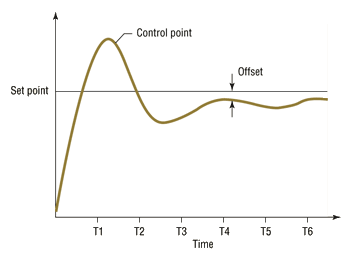
\includegraphics[width=0.5\linewidth]{img/recorrencia-graph.png}
		\label{fig:graph}
		\caption{Representação da atuação do controle sobre o ganho da aceleração e controle de velocidade do carro.}
	\end{figure}



\section{Análise do Funcionamento dos Motores} \label{sec:analitico}
	De forma a adentrar na causa que impediu a conclusão do trabalho, realizou-se testes analíticos a fim de encontrar a causa dos problemas.

	% explicando os intervalos e as situações
	Como o carro necessita de se comportar bem em altas e baixas rotações, analisou-se duas das mais importantes sendo esta quando os motores estão em alta e baixa rotação.% partindo da premissa que o motor inicia-se parado.

	%Para o funcionamento do carro de forma correta, seria necessário o controle proporcional ter gerência de vários intervalos de velocidade, desde a velocidade máxima até a menor, incluindo quando o motor estiver parado. 
	%Ao possuir um intervalo grande de velocidade, permite-se que o carro fizesse curvas com melhor controle evitando as oscilações grandes.
	%Eliminando a situação de quando o motor está parado, para validação, analisou-se das duas ocasiões mais importantes enfrentadas pelo carro, sendo essas quando ele está em alta e baixa rotação. 
	%Esses dados são importantes pelo fato que ambas (alta e baixa rotação) são velocidade extremas do intervalo usado pelo controle e que elas possuem outras variáveis que influenciam na sua atuação como a intensidade da corrente de partida e a resistência dos trens de engrenagem situados em cada motor, por exemplo.

	Para representar essas rotações, foi relacionado os intervalos de valores de PWM da plataforma de protipação. Dessa forma, como o NodeMCU gera um intervalo de 0 à 1023 para valores de PWM, utilizou-se dos valores 1023 e 600 para alta e baixa rotação respectivamente. 
	%O carro que comporte em ambas as situações permite-se concluir que ele possui todos os requisitos físicos necessários para que o controle consiga operar com mais facilidade obtendo melhor precisão em suas tarefas propostas.
	%Assim, o carro que não realizar bem tais movimentos, poderá ter problemas futuros como estabilidade e precisão, por exemplo.

	Neste primeiro teste, partiu-se do princípio que o motor encontra-se parado. Sobre esse aspecto, os itens analisados foram as correntes:

	\begin{description}
		\item [Partida:] Intensidade de corrente que o motor necessita para gerenciar a partida, ou seja, a tentativa de movimento;
		\item [Nominal:] Intensidade de corrente após a tentativa de partida inicial. Valores normativos do motor ao longo do tempo seguindo um mesmo valor de entrada de PWM.
		%\item [Movimento:] Intensidade do motor quando este está realmente realizando o movimento giratório, ou seja, quando realmente conseguiu sair da inércia inicial que é estar sem movimento.
	\end{description}

	Executou-se dez testes mensurando\footnote{Sendo $\bar{X}$ a média, $\sigma$ o desvio padrão e a porcentagem do erro calculado pela fórmula $\frac{\sigma}{\sqrt{|x|}}$ no qual $x$ sendo os total de valores coletados.} os valores de intensidade de corrente em Partida (Tabela \ref{tab:corrente_partida}) e Nominal (Tabela \ref{tab:corrente_nominal}).% e Movimento (Tabela \ref{tab:corrente_rotacionado}).

	\begin{table}[H]
    	\centering
    	\caption{Tabela de valores médios de intensidade de corrente de partida aos principais movimentos requeridos pelo carro robô.}
	    \begin{tabular}{|c||c|c|c|} \hline
	    ~                      & $\bar{X}$ \textbf{Corrente de Partida}   & $\sigma$   & \textbf{\% Erro} \\ \hline \hline
	    \textbf{Alta  Rotação} & $313,7mA$                                & $26,36938$ & $8,338732$    \\ \hline
	    \textbf{Baixa Rotação} & $283,2mA$                                & $19,65706$ & $6,216108$    \\
	     \hline
	    \end{tabular}   \label{tab:corrente_partida}
	\end{table}

	\begin{table}[H]
    	\centering
    	\caption{Tabela de valores médios de intensidade de corrente nominal aos principais movimentos requeridos pelo carro robô.}
	    \begin{tabular}{|c||c|c|c|} \hline
	    ~                      & $\bar{X}$ \textbf{Corrente Nominal} & $\sigma$   & \textbf{\% Erro} \\ \hline \hline
	    \textbf{Alta  Rotação} & $138,9mA$                           & $14,22400$ & $4,498024$     \\ \hline
	    \textbf{Baixa Rotação} & $215,7mA$                           & $11,75727$ & $3,717974$     \\ 
	     \hline
	    \end{tabular}   \label{tab:corrente_nominal}
	\end{table}

	%teste alta velocidade
	%\subsection{Análise da Alta Rotação}
		Olhando primeiramente a alta rotação, o carro possui força suficiente para iniciar seu movimento com a corrente de partida ($313,7mA$) e, depois de vencer a inércia, a corrente estabiliza em valores próximos à $138,9mA$ fazendo o motor girar como estabelecido. 

		Todos os dez testes realizados com este valor de potência fez com que o carro obtivesse teve sucesso para vencer sua inércia inicial. Isso deve-se ao fato da aceleração do motor ser alta, sobrepondo qualquer resistência física que impede o movimento da roda. Diferentemente do teste de alta rotação, o teste com baixa velocidade não obteve tanto sucesso.

	%teste baixa velocidade
	%\subsection{Análise da Baixa Rotação}
		Nos testes de baixa rotação o valor de intensidade de corrente de partida teve uma média de $283,2mA$, mas, em todos os testes realizados, esse valor de potência não foi suficiente para iniciar a rotação no motor. 
		O valor $600$ de PWM fracassou em todos os testes di girar a roda, mesmo o motor demonstrando aplicar a força ao emitir barulho de acionamento. 

		Verificando a dificuldade do início da rotação nos testes de baixa velocidade, foi realizado uma nova medição de valores de corrente nominal com o motor partindo da definição que eles já estávam em movimento. Assim, obteve os resultados da Tabela Movimento (Tabela \ref{tab:corrente_rotacionado}).
		%uma pequena ajuda manual à roda para o giro inicial e percebeu que, para este giro inicial, o motor aplica uma força suficiente para a movimentação do carro mas insuficiente para vencer a resistência dos trens de engrenagens da caixa de redução.


	\begin{table}[H]
    	\centering
    	\caption{Tabela de valores médios de intensidade de corrente com o motor rotacionando aos principais movimentos requeridos pelo carro robô.}
	    \begin{tabular}{|c||c|c|c|} \hline
	    ~                      & $\bar{X}$ \textbf{Corrente c/ Motor em Rotação} & $\sigma$   & \textbf{\% Erro} \\ \hline \hline
	    \textbf{Alta  Rotação} & $142,0mA$                                         & $5,656854$ & $1,788854$     \\ \hline
	    \textbf{Baixa Rotação} & $130,8mA$                                         & $18,68927$ & $5,910067$     \\ 
	     \hline
	    \end{tabular}   \label{tab:corrente_rotacionado}
	\end{table}

	Tabela \ref{tab:corrente_rotacionado} exibe valores mais baixos de corrente nominal partindo do pressuposto de que o motor já estava girando. 
    
	Em teoria, a baixa rotação deveria ser acionada, o motor iniciar seu giro e a rotação estabilizada com valores de intensidade de corrente nominal $I_{nominal} = 130,8$. Entretanto, a corrente de partida $ I_{partida} = 283,2$ não é suficiente para iniciar a movimentação do carro. Dos testes realizados com propósito do motor conseguir dar a partida, necessitou-se de intensidades de correntes maiores que $I_{giro} = 311,1$ para obter seu início. Isso da uma diferença de corrente de $I_{diferenca\_partida} = 27,9mA$, ou seja $10,1505\%$ de potência a mais para as rotações tendo o PWM em valores próximos de $665$.
    
    Na Seção \ref{sec:discussao} será feita uma discussão sobre os dados coletados em relação à atuação do carro.

	\subsection{Discussão} \label{sec:discussao}
		%Após os testes, percebeu-se alguns problemas principais no projeto sendo eles: 1) Resistência das engrenagens da caixa de redução; e 2) Torque fraco dos motores. Eles serão descritos a seguir.

		%  peso do carro
		%O primeiro problema é o \todo{peso} do carro. Ao adicionar todos os componentes para seu funcionamento, percebeu-se que o carro possui \todo{peso} elevado. Os motores possuem força o suficiente para realizar o movimento do carro, mas com \todo{peso} elevado, o controle terá maior dificuldade de controlar a partida dos motores e a estabilização da velocidade.

		\subsubsection{Trens de Engrenagens da Caixa de Redução}
			% engrenagens

			%comparacao
			%Dessa forma, sabendo de tais problemas físicos do carro, realizou-se uma análise das situações mais importantes que o robô enfrenta com base em movimento teóricos perfeitos que fariam o carro realizar a tarefa proposta com sucesso.
			

			Feito a análise de correntes, percebeu-se que existe uma grande resistência das caixas de reduções para início de rotação.
			Esse problema físico foi perceptível ao visualizar a situação na qual o motor injetava potência para iniciar o giro e não conseguia. Pensou-se de início que a potência acionada era insuficiente para a movimentação do carro, entretanto, no teste com o carro já em movimento, o valor mostrou-se suficiente para mover o carro com todos os componentes instalados com facilidade. Assim, a potência é suficiente para arrastar o carro, mas não para dar sua partida.
			Houve situações de execução fora dos testes em que o carro injetou potência máxima nos motores (valor $1023$ de PWM) e eles não conseguiam se mover.

			% problema da engrenagens resolvidas pelo controle
			Esse problema poderia ser resolvido pelo controle, acionando mais potência no início e depois equilibrando no início de seu movimento. Entretanto, esse procedimento não foi possível ser implementado por vários motivos sendo eles:

			\begin{enumerate}
				\item Injetar mais potência na partida faz com que sua aceleração seja alta de tal forma que, após iniciada, o controle não consiga corrigí-la. Isso é causado pelo item mencionado em Seção \ref{sec:problema_motor} no qual é descrito um certo atraso na atuação do motor, podendo causar descontrole de seus movimentos e consequentemente a perdendo o caminho a seguir. Sendo assim, a primeira solução sobre o problema da resistência foi adicionar mais pares de motores ao carro, entretanto, o chassi do carro não possui suporte para a instalação de mais motores com seus \textit{encoders};

				% valores altos de potência fazem o carrinho perder o controle
				\item O carro ter que percorrer $9\degree$ (ou seja, $0,5105$ centímetros) para que o controle note o início do movimento também é um fator que torna o problema complexo. 
				Essa distância percorrida somada com o tempo processamento do carro ($30$ milissegundos), do processamento da nuvem e sua a latência de comunicação de envio e do recebimento de dados até a atuação do controle faz com que o carro percorra cerca de $0,742$ centímetros até que a atuação seja totalmente completada. 
				
                Esse valor de distância é suficiente para fazer com que o carro não consiga recuperar de uma situação que exija mais potencial do controle. O problema poderia apresentar uma solução ao utilizar um disco para \textit{encoder} com mais vasos criando uma precisão maior dos movimentos, mas não havia tal equipamento para uso. Esse problema de controle de aceleração torna mais problemático ainda no carro $ \mathcal{B} $ pois:

				\begin{itemize}
					\item Como ele não possui um item de controle de posição geral de trajeto, o carro fica a mercê da precisão exercida pelo controle junto com os valores obtidos com o \textit{encoder}. Com um controle de aceleração dado pelos fatores acima, cada movimento do carro acumula erros exponencialmente. De uma maneira mais geral, a cada movimento é gerado um erro que é aplicado no próximo movimento e assim gerado um novo erro com valor exponencialmente maior, criando assim uma bola de neve e inviabilizando a reprodução do carro $ \mathcal{B} $.
				\end{itemize}
			\end{enumerate}


\section{Conclusão} \label{sec:conclusao}

	Como produto do trabalho, o carro $ \mathcal{A} $ consegue completar o trajeto com algumas dificuldades mesmo o processamento situar todo em nuvem. Entretanto, o carro $ \mathcal{B} $ não conseguiu realizar nenhuma vez sua tarefa de reprodução do trajeto realizado por $ \mathcal{A} $. Isso pois não foi possível neste trabalho a construção de um modelo que levasse em consideração o fator de erro do $ \mathcal{B} $ em relação ao trajeto.

	Como demostrativo do funcionamento do carro $ \mathcal{A} $, segue os \textit{links} disponibilizou-se três vídeos para exemplificar o funcionamento do carro. O primeiro vídeo \url{https://youtu.be/RWjgYUrU1Fo} exibe o carro realizando seu dever de completar o trajeto. O mesmo vídeo pode ser visto em câmera lenta, gravado em $240fps$ percebendo cada detalhe do carro e seu procedimento de controle, disponível em \url{https://youtu.be/xk-tbqkAVOs}. Também foi disponibilizado um vídeo demonstrando o tempo de demora na atuação dos motores após a leitura da faixa no qual pode ser verificado em câmera lenta, disponibilizado em \url{https://youtu.be/pGvHHe4h54I}. Por fim, outro vídeo (com música de fundo) demonstrando outra atuação do carro, disponível em \url{https://youtu.be/SD5c9YnoTfo}. Como mencionado, não há demonstração do carro $ \mathcal{B} $ pois todos os testes realizados com tal foram falhos.

	% tempo de resposta
    Após analisado os componentes em conjunto com a atuação do controle proporcional do carro, percebeu-se que a latência de resposta do motor em virtude ao intervalo de resposta esperado pelo controle faz com que o carro não tenha uma precisão fina sobre seus movimentos. Esse problema poderia ser reduzido ao utilizar abordagem que passasse a utilizar um processamento de controle totalmente local tornando o processamento mais preciso.
    
	% mais tricks seria legal
	Utilizar um \textit{encoder} que contenha mais vasos faz com que seja criado uma maior percepção de movimento, fazendo com que o controle gerencie melhor a velocidade do carro. 
    O modelo atual utilizado usa apenas 3 valores de velocidade pelo fato do tempo curto de captura de taxa de variação de \textit{tricks} criando curta amostra de velocidade. Com um disco com mais vasos, é possível multiplicar o nível de precisão de seus movimentos.

	% engrenagens
	Mesmo com torque suficiente para mover-se em baixas rotações, o motor não conseguiu vencer à resistência dos trilhos de engrenagens em situações onde o carro encontrava-se estacionado. Como mencionado na Seção \ref{sec:discussao}, aumentar a aceleração de fato faz o carro dar a partida, mas isso acarreta vários outros problemas relacionados a aceleração. Para garantir acelerações suaves, seria necessário utilizar um sistema de engrenagens que não obtivesse tanta resistência ou motores que tivesse uma capacidade de torque maior.

	% peso}
	%Obviamente, utilizar componentes mais leves faz com que o carro tenha mais facilidade de movimentação dispondo menos resistência aos motores. Quanto menor a resistência enfrentadas pelos motores, mais será a eficiência energética e e seu fator de controle.

	% novo chassi
	%Propor um trabalho fornecendo um chassi que tenha suporte à mais motores e seus \textit{encoders} faz com que o trabalho possa ser desmembrado em mais opções de construções. Alterar a estrutura física do carro, adicionando mais motores por exemplo, faz com que o desenvolvimento do carro seja abordado de mais formas, escolhendo a que mais atrela ao ambiente testado e equipamentos disponibilizados.


	%O carro $ \mathcal{A} $ consegue completar o trajeto com muita dificuldade pela quantidade de sensores que o carro possui, incluindo seus chassis, rodas, motores, controlador etc. A fim de contornar esse problema, implementou-se um controlador que fosse capaz de lidar com esse problema de atuação dos motores obrigando o carro parar a cada momento que encontra uma faixa, já que este fica impossibilitado de movimentar mesmo utilizando dois \textit{packs} de pilhas com um total de $6V$ cada. 

	% dificuldades
    \subsection{Dificuldades e Ganhos de Aprendizagem}
	Todos os dois \textit{motor shield} fornecidos para o trabalho possuíam problema de circuito físico no qual, o seu componente \textit{not}, que permitia o motor girar em sentido contrário, estavam danificados. Não se sabe o motivo da danificação. Gastou-se muito tempo descobrindo a falta deste circuito integrado e por isso o projeto foi fundado sobre o \textit{motor shield} incapacitado de girar os motores em sentido reverso.

	A geração de um mapa para o carro $ \mathcal{B} $ também foi uma tarefa incompleta. Realizou-se várias tentativas de geração e reprodução de mapas utilizando várias combinações de sensores, mas todas foram fracassadas.

	% Utilização de controles mais eficientes
	O controle proporcional (P) desenvolvido neste trabalho foi capaz de concluir o objetivo do carro $ \mathcal{A} $ mas com dificuldade. É possível realizar um novo estudo a fim de utilizar controle proporcional integral-derivativo (PID) a fim de aprimorar os movimentos dos carros.

	% ganhos
	Neste trabalho foi possível perceber a importância dos controles proporcionais de primeira ordem. Este exemplo de \textit{follow line} do trabalho mostrou-se claro ao comparar as vantagens de sua utilização para obter melhores resultados na sua tarefa. 
    Esse trabalho tornou-se extremamente útil na percepção da qual vários outros sistemas poderiam tomar proveito do uso de tais ferramentas para controle de suas tarefas com maior precisão.
	Outro tópico também aprendido na realização deste trabalho foi o aperfeiçoamento das técnicas básicas de confecção, manuseio e aferição de circuitos eletrônicos simples. Foi necessário conhecimentos básicos sobre corrente elétrica, teoria de circuitos eletrônicos e operação com algumas funcionalidades do multímetro para a construção do trabalho.